\section{V. Thống kê suy diễn.}
\label{v.-thux1ed1ng-kuxea-suy-diux1ec5n.}

\subsection{1. Bài toán 1 mẫu }

\textbf{Bài toán:} Với mức ý nghĩa 5\%, cho kết luận độ nhám trung bình
của bản in là 170 µm hay không?

\emph{Kiểm tra giả định về phân phối chuẩn cho biến độ nhám: }

\begin{Shaded}
\begin{Highlighting}[]
\FunctionTok{qqnorm}\NormalTok{(data}\SpecialCharTok{$}\NormalTok{roughness)}
\FunctionTok{qqline}\NormalTok{(data}\SpecialCharTok{$}\NormalTok{roughness, }\AttributeTok{col =} \StringTok{"red"}\NormalTok{)}
\end{Highlighting}
\end{Shaded}

\begin{figure}[htbp]
    \centering
    \pandocbounded{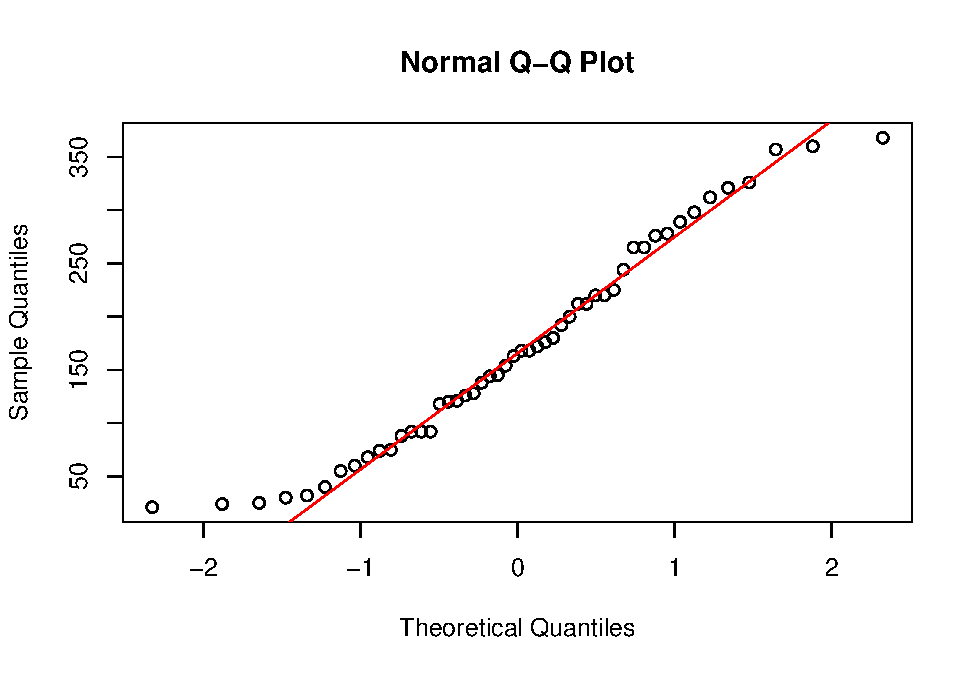
\includegraphics[keepaspectratio]{unnamed-chunk-10-1.pdf}}
    \caption{Đồ thị Q-Q Plot kiểm tra phân phối chuẩn của độ nhám bề mặt}
    \label{fig:qq_roughness}
\end{figure}
\newpage

\textbf{Nhận xét:}

Dựa vào đồ thị ta nhận thấy đa số các quan trắc nằm xung quanh đường
thẳng kì vọng phân phối chuẩn, ta có thể kết luận rằng độ nhám có phân
phối chuẩn.

\emph{Ngoài ra, ta có thể dùng kiểm định \texttt{shapiro.test} để kiểm
tra: }

\begin{itemize}
\tightlist
\item
  Giả thiết \(H_0\): Độ nhám tuân theo phân phối chuẩn
\item
  Giả thiết \(H_1\): Độ nhám không tuân theo phân phối chuẩn
\end{itemize}

\begin{Shaded}
\begin{Highlighting}[]
\FunctionTok{shapiro.test}\NormalTok{(new\_data}\SpecialCharTok{$}\NormalTok{roughness)}
\end{Highlighting}
\end{Shaded}

\begin{verbatim}
## 
##  Shapiro-Wilk normality test
## 
## data:  new_data$roughness
## W = 0.95919, p-value = 0.08221
\end{verbatim}

\textbf{Nhận xét: }

Vì \texttt{p-value\ =\ 0.08221} \textgreater{} mức ý nghĩa 5\% nên ta
chưa bác bỏ được \(H_0\).

Vậy ta có thể kết luận rằng độ nhám có phân phối chuẩn.

\(\Rightarrow\) Đây là dạng bài kiểm định trung bình 1 mẫu, X có phân phối chuẩn, chưa
biết \(\sigma_2\)

Gọi \(\mu\) là độ nhám trung bình của bản in thực tế. - Giả thiết
\(H_0: \mu = 170\) - Giả thiết \(H_1: \mu \neq 170\)

\emph{Thực hiện kiểm định bằng \texttt{t-test}:}

\begin{Shaded}
\begin{Highlighting}[]
\FunctionTok{t.test}\NormalTok{(new\_data}\SpecialCharTok{$}\NormalTok{roughness, }\AttributeTok{mu =} \DecValTok{170}\NormalTok{)}
\end{Highlighting}
\end{Shaded}

\begin{verbatim}
## 
##  One Sample t-test
## 
## data:  new_data$roughness
## t = 0.041412, df = 49, p-value = 0.9671
## alternative hypothesis: true mean is not equal to 170
## 95 percent confidence interval:
##  142.4348 198.7252
## sample estimates:
## mean of x 
##    170.58
\end{verbatim}

\textbf{Nhận xét:} Vì \texttt{p-value\ =\ 0.9671} \textgreater{} mức ý
nghĩa 5\% nên ta chưa bác bỏ được \(H_0\).

Vậy nên ta có thể kết luận độ nhám trung bình của bản in là 170 µm, xét
mức ý nghĩa 5\%

\emph{Ngoài ra ta có thể đưa ra kết luận bằng cách:}

Tiêu chuẩn kiểm định \(t_0 = 0.0414\).

Miền bác bỏ:
\(RR = (-\infty; -t_{\alpha/2; n-1}) \cup (t_{\alpha/2; n-1}; +\infty)\)

Với \(t_{\alpha/2; n-1}\) được tính bằng công thức:

\begin{Shaded}
\begin{Highlighting}[]
\FunctionTok{qt}\NormalTok{(}\AttributeTok{p =} \FloatTok{0.05}\SpecialCharTok{/}\DecValTok{2}\NormalTok{, }\AttributeTok{df =} \FunctionTok{nrow}\NormalTok{(new\_data)}\SpecialCharTok{{-}}\DecValTok{1}\NormalTok{, }\AttributeTok{lower.tail =} \ConstantTok{FALSE}\NormalTok{)}
\end{Highlighting}
\end{Shaded}

\begin{verbatim}
## [1] 2.009575
\end{verbatim}

\(RR = (-\infty; -2.0096) \cup (2.0096; +\infty)\)

Vì \(t_0 \notin RR\) nên ta chưa bác bỏ \(H_0\).

Vậy \emph{ta có thể kết luận độ nhám trung bình của bản in là 170 µm,
xét mức ý nghĩa 5\%}.

\subsection{2. Kiểm định 2 mẫu.}

\textbf{Bài toán:} Với mức ý nghĩa 0.05\%, hãy so sánh độ nhám trung
bình của bản in khi sử dụng vật liệu abs và pla.

\begin{itemize}
\tightlist
\item
  Chia bộ dữ liệu theo 2 nhóm vật liệu:
\end{itemize}

\begin{Shaded}
\begin{Highlighting}[]
\NormalTok{abs\_data }\OtherTok{\textless{}{-}} \FunctionTok{subset}\NormalTok{(data, material }\SpecialCharTok{==} \StringTok{"abs"}\NormalTok{)}
\NormalTok{pla\_data }\OtherTok{\textless{}{-}} \FunctionTok{subset}\NormalTok{(data, material }\SpecialCharTok{==} \StringTok{"pla"}\NormalTok{)}
\end{Highlighting}
\end{Shaded}

\emph{Kiểm tra giả định về phân phối chuẩn cho biến độ nhám ở loại vật
liệu abs:}

\begin{Shaded}
\begin{Highlighting}[]
\FunctionTok{qqnorm}\NormalTok{(abs\_data}\SpecialCharTok{$}\NormalTok{roughness); }\FunctionTok{qqline}\NormalTok{(abs\_data}\SpecialCharTok{$}\NormalTok{roughness, }\AttributeTok{col =} \StringTok{"red"}\NormalTok{)}
\end{Highlighting}
\end{Shaded}

\begin{figure}[htbp]
    \centering
    \pandocbounded{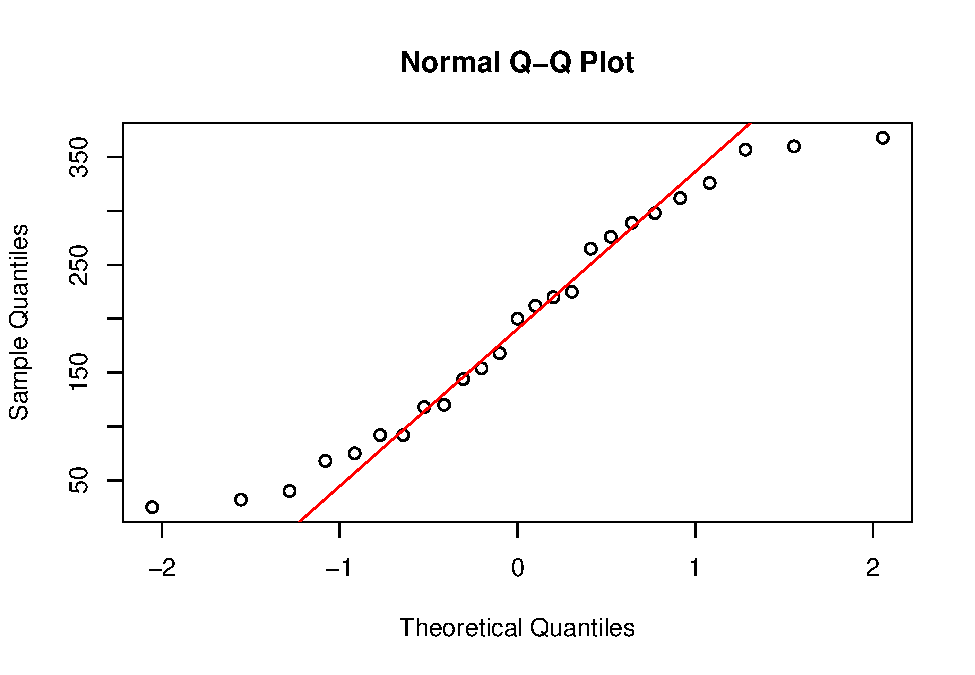
\includegraphics[keepaspectratio]{unnamed-chunk-15-1.pdf}}
    \caption{Đồ thị Q-Q Plot kiểm tra phân phối chuẩn của độ nhám với vật liệu ABS}
    \label{fig:qq_abs}
\end{figure}

\textbf{Nhận xét:}

Dựa vào đồ thị ta nhận thấy đa số các quan trắc nằm xung quanh đường
thẳng kì vọng phân phối chuẩn, ta có thể kết luận rằng độ nhám ở vật
liệu abs có phân phối chuẩn.

\emph{Ngoài ra, ta có thể dùng kiểm định \texttt{shapiro.test} để kiểm
tra:}

\begin{itemize}
\tightlist
\item
  Giả thiết \(H_0: \sigma_1^2 = \sigma_2^2\) hay
  \((\sigma_1^2 \leq \sigma_2^2)\)
\item
  Giả thiết \(H_1: \sigma_1^2 > \sigma_2^2\)
\end{itemize}

\begin{Shaded}
\begin{Highlighting}[]
\FunctionTok{shapiro.test}\NormalTok{(abs\_data}\SpecialCharTok{$}\NormalTok{roughness)}
\end{Highlighting}
\end{Shaded}

\begin{verbatim}
## 
##  Shapiro-Wilk normality test
## 
## data:  abs_data$roughness
## W = 0.94235, p-value = 0.1677
\end{verbatim}

\textbf{Nhận xét:} Vì \texttt{p-value\ =\ 0.1677} \textgreater{} mức ý
nghĩa 5\% nên ta chưa bác bỏ được \(H_0\).

Vậy ta có thể kết luận rằng độ nhám ở vật liệu abs có phân phối chuẩn.

\emph{Kiểm tra giả định về phân phối chuẩn cho biến độ nhám ở loại vật
liệu pla:}

\begin{Shaded}
\begin{Highlighting}[]
\FunctionTok{qqnorm}\NormalTok{(pla\_data}\SpecialCharTok{$}\NormalTok{roughness); }\FunctionTok{qqline}\NormalTok{(pla\_data}\SpecialCharTok{$}\NormalTok{roughness, }\AttributeTok{col =} \StringTok{"red"}\NormalTok{)}
\end{Highlighting}
\end{Shaded}

\begin{figure}[htbp]
    \centering
    \pandocbounded{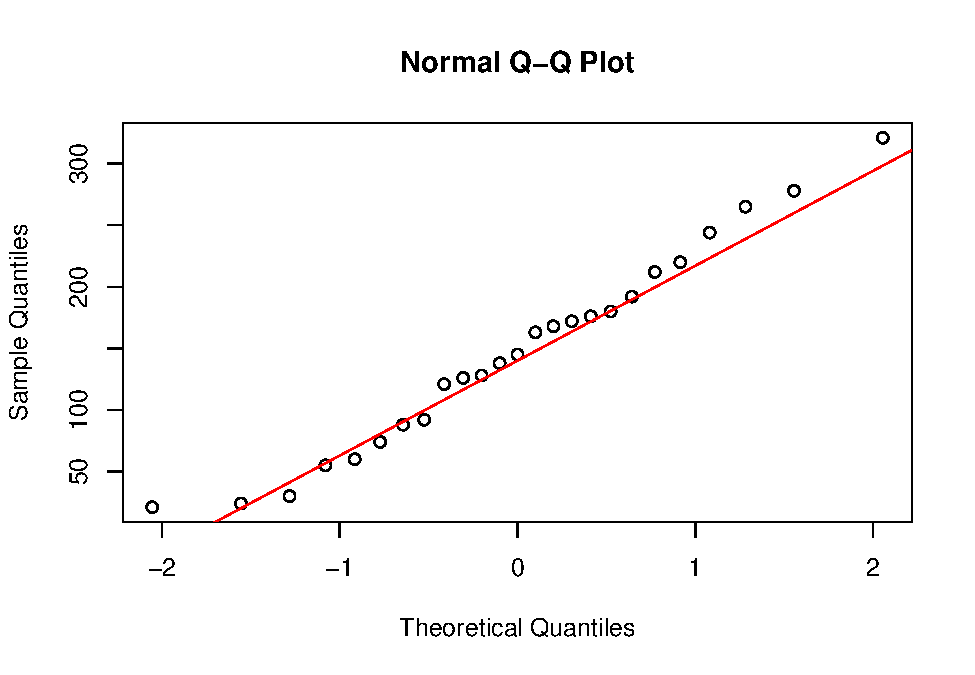
\includegraphics[keepaspectratio]{unnamed-chunk-17-1.pdf}}
    \caption{Đồ thị Q-Q Plot kiểm tra phân phối chuẩn của độ nhám với vật liệu PLA}
    \label{fig:qq_pla}
\end{figure}
\newpage

\textbf{Nhận xét:}

Dựa vào đồ thị ta nhận thấy đa số các quan trắc nằm xung quanh đường
thẳng kì vọng phân phối chuẩn, ta có thể kết luận rằng độ nhám ở vật
liệu pla có phân phối chuẩn.

\emph{Ngoài ra, ta có thể dùng kiểm định shapiro.test để kiểm tra:}

\begin{itemize}
\tightlist
\item
  Giả thiết \(H_0\): Độ nhám ở vật liệu pla tuân theo phân phối chuẩn
\item
  Giả thiết \(H_1\): Độ nhám ở vật liệu pla không tuân theo phân phối chuẩn
\end{itemize}

\begin{Shaded}
\begin{Highlighting}[]
\FunctionTok{shapiro.test}\NormalTok{(pla\_data}\SpecialCharTok{$}\NormalTok{roughness)}
\end{Highlighting}
\end{Shaded}

\begin{verbatim}
## 
##  Shapiro-Wilk normality test
## 
## data:  pla_data$roughness
## W = 0.97437, p-value = 0.7561
\end{verbatim}

\textbf{Nhận xét:} Vì \texttt{p-value\ =\ 0.1677} \textgreater{} mức ý
nghĩa 5\% nên ta chưa bác bỏ được \(H_0\).

Vậy ta có thể kết luận rằng độ nhám ở vật liệu pla có phân phối chuẩn.

\emph{Thực hiện so sánh phương sai độ nhám ở 2 nhóm vật liệu: }

\begin{itemize}
\item
  Giả thiết \(H_0: \sigma_1^2=  \sigma_2^2\) hay
  \((\sigma_1^2≤ \sigma_2^2)\)
\item
  Giả thiết \(H_1: \sigma_1^2> \sigma_2^2\)
\end{itemize}

\begin{Shaded}
\begin{Highlighting}[]
\FunctionTok{var.test}\NormalTok{(abs\_data}\SpecialCharTok{$}\NormalTok{roughness, pla\_data}\SpecialCharTok{$}\NormalTok{roughness, }\AttributeTok{alternative =} \StringTok{"greater"}\NormalTok{)}
\end{Highlighting}
\end{Shaded}

\begin{verbatim}
## 
##  F test to compare two variances
## 
## data:  abs_data$roughness and pla_data$roughness
## F = 1.8454, num df = 24, denom df = 24, p-value = 0.07024
## alternative hypothesis: true ratio of variances is greater than 1
## 95 percent confidence interval:
##  0.9302656       Inf
## sample estimates:
## ratio of variances 
##           1.845423
\end{verbatim}

\textbf{Nhận xét:} Vì \texttt{p-value\ =\ 0.07024} \textgreater{} mức ý
nghĩa 5\% nên ta chưa bác bỏ được H\_0.

Vậy phương sai độ nhóm ở 2 nhóm vật liệu bằng nhau.

⇨ Đây là dạng bài kiểm định trung bình 2 mẫu độc lập , X1, X2 có phân phối chuẩn, chưa biết \(\sigma_1^2, \sigma_2^2\) với \(\sigma_1^2=  \sigma_2^2\)

Gọi \(\mu_1 , \mu_2 \) lần lượt là độ nhám trung bình của bản in khi sử dụng vật liệu
abs và pla.

\begin{itemize}
\tightlist
\item
  Giả thiết \(H_0: \mu_1 = \mu_2\)\\
\item
  Giả thiết \(H_1: \mu_1 > \mu_2\)
\end{itemize}

\emph{Thực hiện kiểm định bằng t-test: }

\begin{Shaded}
\begin{Highlighting}[]
\FunctionTok{t.test}\NormalTok{(roughness }\SpecialCharTok{\textasciitilde{}}\NormalTok{ material, }\AttributeTok{data =}\NormalTok{ data, }\AttributeTok{alternative =} \StringTok{"greater"}\NormalTok{, }\AttributeTok{var.equal =} \ConstantTok{TRUE}\NormalTok{)}
\end{Highlighting}
\end{Shaded}

\begin{verbatim}
## 
##  Two Sample t-test
## 
## data:  roughness by material
## t = 1.6613, df = 48, p-value = 0.05159
## alternative hypothesis: true difference in means between group abs and group pla is greater than 0
## 95 percent confidence interval:
##  -0.4392901        Inf
## sample estimates:
## mean in group abs mean in group pla 
##            193.44            147.72
\end{verbatim}

\textbf{Nhận xét:} Vì \texttt{p-value\ =\ 0.05159} \textgreater{} mức ý
nghĩa 5\% nên ta chưa bác bỏ được \(H_0\).

Vậy nên độ nhám trung bình ở 2 nhóm vật liệu bằng nhau, xét với mức ý
nghĩa 5\%.

\subsection{3. Bài toán phân tích phương sai}

\subsubsection{3.1. Tính toán các giá trị}

\textbf{Bài toán:} So sánh độ nhám trung bình ở 5 nhóm
\texttt{layer\_height}.

\textbf{Phân tích:} ANOVA là bài toán so sánh trung bình của các tổng
thể nhưng với yêu cầu mỗi biến ảnh hưởng phải có 3 phân loại trở lên.

Trong tập dữ liệu ta có 2 biến phân loại là \texttt{infill\_patten} và
\texttt{material} nhưng mỗi biến thì chỉ có 2 phân loại là biến
\texttt{infill\_pattern} bao gồm \texttt{grid} và \texttt{honeycomb},
biến \texttt{materia}l bao gồm \texttt{pla} và \texttt{abs}.

\(\Rightarrow\) Giải pháp: Dùng biến \texttt{layer\_heght} và chia các giá trị thành
các nhóm.

\begin{Shaded}
\begin{Highlighting}[]
\NormalTok{data}\SpecialCharTok{$}\NormalTok{layer\_height }\OtherTok{\textless{}{-}} \FunctionTok{as.factor}\NormalTok{(data}\SpecialCharTok{$}\NormalTok{layer\_height)}
\FunctionTok{print}\NormalTok{(data}\SpecialCharTok{$}\NormalTok{layer\_height)}
\end{Highlighting}
\end{Shaded}

\begin{verbatim}
##  [1] 0.02 0.02 0.02 0.02 0.02 0.02 0.02 0.02 0.02 0.02 0.06 0.06 0.06 0.06 0.06
## [16] 0.06 0.06 0.06 0.06 0.06 0.1  0.1  0.1  0.1  0.1  0.1  0.1  0.1  0.1  0.1 
## [31] 0.15 0.15 0.15 0.15 0.15 0.15 0.15 0.15 0.15 0.15 0.2  0.2  0.2  0.2  0.2 
## [46] 0.2  0.2  0.2  0.2  0.2 
## Levels: 0.02 0.06 0.1 0.15 0.2
\end{verbatim}

Lúc này các giá trị trong biến \texttt{layer\_height} đã được chuyển
sang dạng factor để phân loại.

Biến \texttt{layer\_height} đã có 5 nhóm lần lượt là: \texttt{0.02},
\texttt{0.06}, \texttt{0.1}, \texttt{0.15}, \texttt{0.2}. Đặt giả thuyết

\(H_0: \mu_1=\mu_2=\mu_3=\mu_4=\mu_5\)

\(H_1\): Tồn tại \(\mu_i \neq \mu_j (i\neq j)\)

\emph{Code thực hiện hàm anova, ta sử dụng hàm \texttt{aov()} để tính
toán các giá trị.}

\begin{Shaded}
\begin{Highlighting}[]
\NormalTok{anova\_model }\OtherTok{\textless{}{-}} \FunctionTok{aov}\NormalTok{(roughness }\SpecialCharTok{\textasciitilde{}}\NormalTok{ layer\_height, data)}
\FunctionTok{summary}\NormalTok{(anova\_model)}
\end{Highlighting}
\end{Shaded}

\begin{verbatim}
##              Df Sum Sq Mean Sq F value   Pr(>F)    
## layer_height  4 326957   81739   23.94 1.17e-10 ***
## Residuals    45 153624    3414                     
## ---
## Signif. codes:  0 '***' 0.001 '**' 0.01 '*' 0.05 '.' 0.1 ' ' 1
\end{verbatim}

Ta thấy giá trị của \texttt{Pr(\textgreater{}F)\ =\ 1.17e-10} nhỏ hơn
mức ý nghĩa 5\%

\(\Rightarrow\) Bác bỏ \(H_0\), chấp nhận \(H_1\)

\(\Rightarrow\) Có sự khác biệt về độ nhám trung bình giữa 5 nhóm chiều cao trong biến
\texttt{layer\_height}.

\subsubsection{3.2. Kiểm tra điều kiện mô hình ANOVA }

Điều kiện thứ nhất:

\begin{itemize}
\item
  Các quan sát từ các tổng thể dược lấy độc lập.
\item
  Các giá trị độ nhám trong dự liệu phải được lấy độc lập.
\item
  Điều kiện thứ nhất là hiển nhiên thỏa mãn do mỗi đơn vị dữ liệu được
  thu thập sau mỗi lần in.
\end{itemize}

Điều kiện thứ hai:

\begin{itemize}
\item
  Các tổng thể phải có phân phối chuẩn
\item
  Độ nhám ở các nhóm có phân phối chuẩn.
\end{itemize}

\begin{Shaded}
\begin{Highlighting}[]
\NormalTok{data\_0}\FloatTok{.02} \OtherTok{\textless{}{-}} \FunctionTok{subset}\NormalTok{(data, layer\_height}\SpecialCharTok{==}\StringTok{"0.02"}\NormalTok{)}
\NormalTok{data\_0}\FloatTok{.06} \OtherTok{\textless{}{-}} \FunctionTok{subset}\NormalTok{(data, layer\_height}\SpecialCharTok{==}\StringTok{"0.06"}\NormalTok{)}
\NormalTok{data\_0}\FloatTok{.1} \OtherTok{\textless{}{-}} \FunctionTok{subset}\NormalTok{(data, layer\_height}\SpecialCharTok{==}\StringTok{"0.1"}\NormalTok{)}
\NormalTok{data\_0}\FloatTok{.15} \OtherTok{\textless{}{-}} \FunctionTok{subset}\NormalTok{(data, layer\_height}\SpecialCharTok{==}\StringTok{"0.15"}\NormalTok{)}
\NormalTok{data\_0}\FloatTok{.2} \OtherTok{\textless{}{-}} \FunctionTok{subset}\NormalTok{(data, layer\_height}\SpecialCharTok{==}\StringTok{"0.2"}\NormalTok{)}
\end{Highlighting}
\end{Shaded}

Ta tách các nhóm dữ liệu ra từng tập dữ liệu riêng sau đó dùng hàm
\texttt{qqnorm}, \texttt{qqline} và \texttt{shapiro.test} để kiểm tra.

\emph{data\_0.02}

\begin{Shaded}
\begin{Highlighting}[]
\FunctionTok{qqnorm}\NormalTok{(data\_0}\FloatTok{.02}\SpecialCharTok{$}\NormalTok{roughness, }\AttributeTok{main =} \StringTok{"Q{-}Q Plot data\_0.02 Roughness"}\NormalTok{)}
\FunctionTok{qqline}\NormalTok{(data\_0}\FloatTok{.02}\SpecialCharTok{$}\NormalTok{roughness)}
\end{Highlighting}
\end{Shaded}

\begin{figure}[htbp]
    \centering
    \pandocbounded{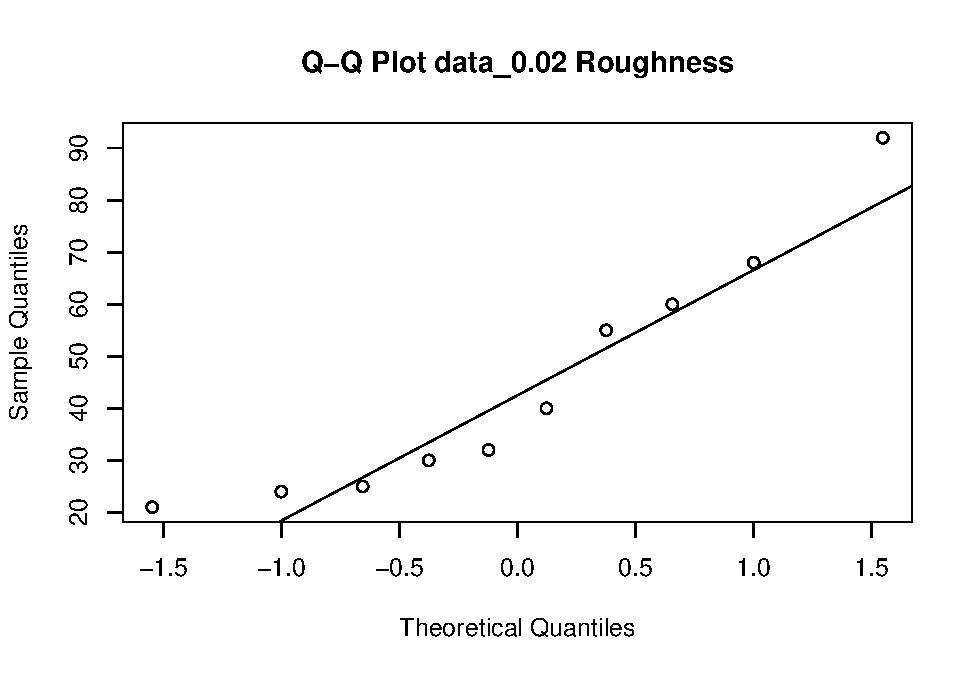
\includegraphics[keepaspectratio]{unnamed-chunk-24-1.pdf}}
    \caption{Đồ thị Q-Q Plot kiểm tra phân phối chuẩn tại chiều cao lớp in 0.02 mm}
    \label{fig:qq_layer_02}
\end{figure}
\newpage

\begin{Shaded}
\begin{Highlighting}[]
\FunctionTok{shapiro.test}\NormalTok{(data\_0}\FloatTok{.02}\SpecialCharTok{$}\NormalTok{roughness)}
\end{Highlighting}
\end{Shaded}

\begin{verbatim}
## 
##  Shapiro-Wilk normality test
## 
## data:  data_0.02$roughness
## W = 0.89205, p-value = 0.1788
\end{verbatim}

\emph{data\_0.06}

\begin{Shaded}
\begin{Highlighting}[]
\FunctionTok{qqnorm}\NormalTok{(data\_0}\FloatTok{.06}\SpecialCharTok{$}\NormalTok{roughness, }\AttributeTok{main =} \StringTok{"Q{-}Q Plot data\_0.06 Roughness"}\NormalTok{) }
\FunctionTok{qqline}\NormalTok{(data\_0}\FloatTok{.06}\SpecialCharTok{$}\NormalTok{roughness)}
\end{Highlighting}
\end{Shaded}

\begin{figure}[htbp]
    \centering
    \pandocbounded{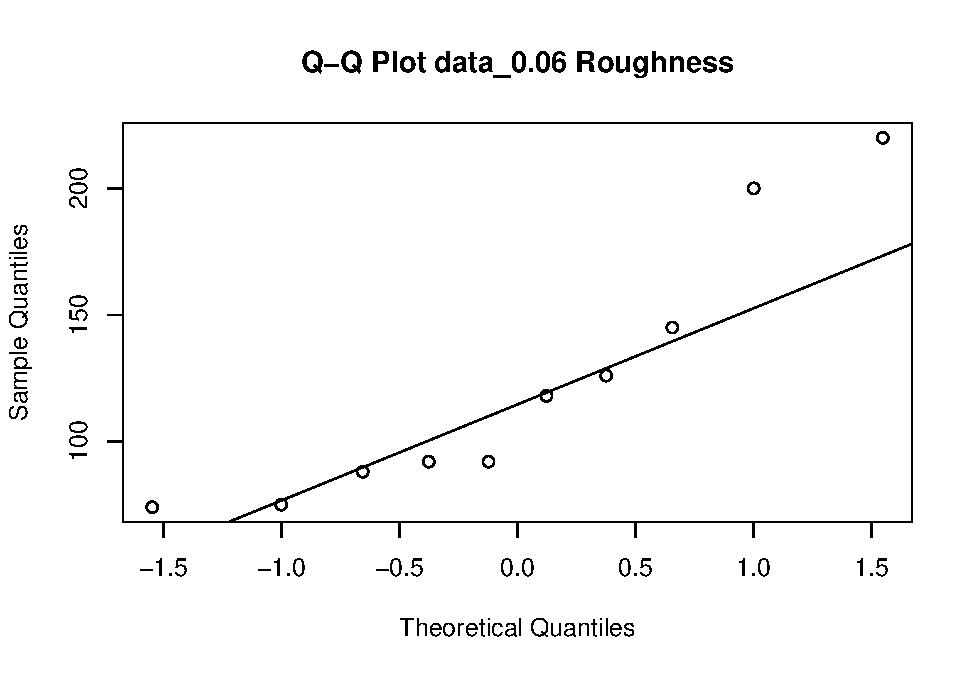
\includegraphics[keepaspectratio]{unnamed-chunk-25-1.pdf}}
    \caption{Đồ thị Q-Q Plot kiểm tra phân phối chuẩn tại chiều cao lớp in 0.06 mm}
    \label{fig:qq_layer_06}
\end{figure}
\newpage

\begin{Shaded}
\begin{Highlighting}[]
\FunctionTok{shapiro.test}\NormalTok{(data\_0}\FloatTok{.06}\SpecialCharTok{$}\NormalTok{roughness)}
\end{Highlighting}
\end{Shaded}

\begin{verbatim}
## 
##  Shapiro-Wilk normality test
## 
## data:  data_0.06$roughness
## W = 0.85434, p-value = 0.0654
\end{verbatim}

\emph{data\_0.1}

\begin{Shaded}
\begin{Highlighting}[]
\FunctionTok{qqnorm}\NormalTok{(data\_0}\FloatTok{.1}\SpecialCharTok{$}\NormalTok{roughness, }\AttributeTok{main =} \StringTok{"Q{-}Q Plot data\_0.1 Roughness"}\NormalTok{)}
\FunctionTok{qqline}\NormalTok{(data\_0}\FloatTok{.1}\SpecialCharTok{$}\NormalTok{roughness)}
\end{Highlighting}
\end{Shaded}

\begin{figure}[htbp]
    \centering
    \pandocbounded{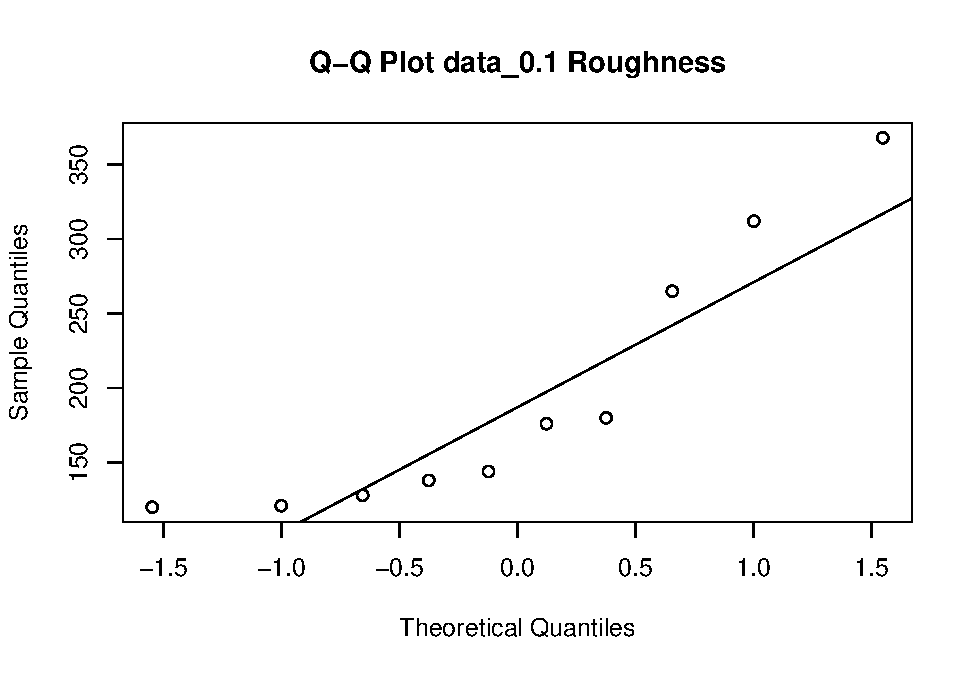
\includegraphics[keepaspectratio]{unnamed-chunk-26-1.pdf}}
    \caption{Đồ thị Q-Q Plot kiểm tra phân phối chuẩn tại chiều cao lớp in 0.1 mm}
    \label{fig:qq_layer_1}
\end{figure}
\newpage

\begin{Shaded}
\begin{Highlighting}[]
\FunctionTok{shapiro.test}\NormalTok{(data\_0}\FloatTok{.1}\SpecialCharTok{$}\NormalTok{roughness)}
\end{Highlighting}
\end{Shaded}

\begin{verbatim}
## 
##  Shapiro-Wilk normality test
## 
## data:  data_0.1$roughness
## W = 0.82279, p-value = 0.02739
\end{verbatim}

\emph{data\_0.15}

\begin{Shaded}
\begin{Highlighting}[]
\FunctionTok{qqnorm}\NormalTok{(data\_0}\FloatTok{.15}\SpecialCharTok{$}\NormalTok{roughness, }\AttributeTok{main =} \StringTok{"Q{-}Q Plot data\_0.15 Roughness"}\NormalTok{)}
\FunctionTok{qqline}\NormalTok{(data\_0}\FloatTok{.15}\SpecialCharTok{$}\NormalTok{roughness)}
\end{Highlighting}
\end{Shaded}

\begin{figure}[htbp]
    \centering
    \pandocbounded{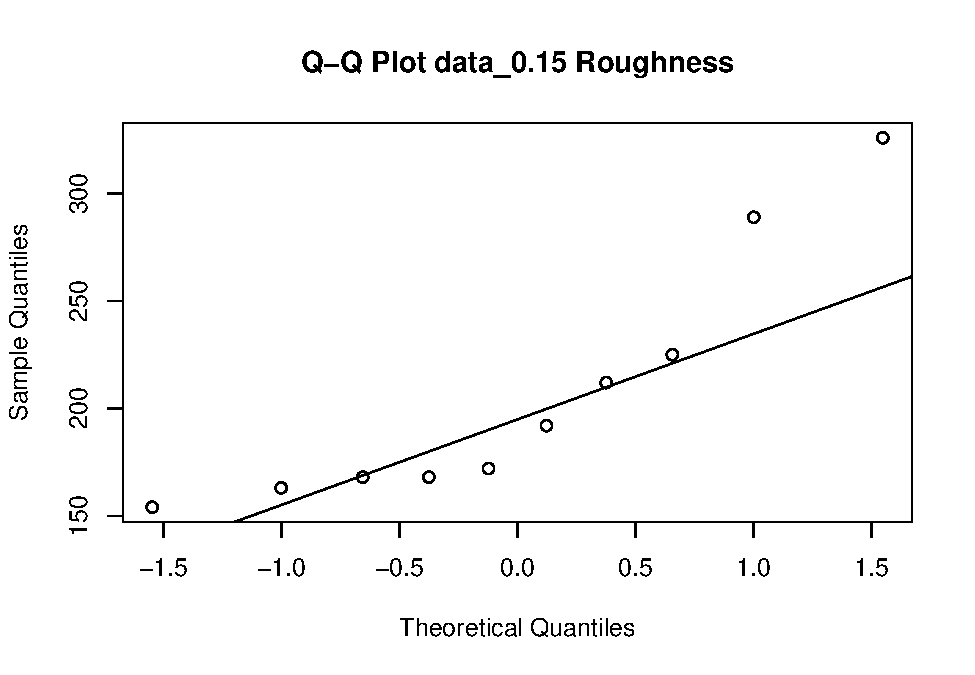
\includegraphics[keepaspectratio]{unnamed-chunk-27-1.pdf}}
    \caption{Đồ thị Q-Q Plot kiểm tra phân phối chuẩn tại chiều cao lớp in 0.15 mm}
    \label{fig:qq_layer_15}
\end{figure}
\newpage

\begin{Shaded}
\begin{Highlighting}[]
\FunctionTok{shapiro.test}\NormalTok{(data\_0}\FloatTok{.15}\SpecialCharTok{$}\NormalTok{roughness)}
\end{Highlighting}
\end{Shaded}

\begin{verbatim}
## 
##  Shapiro-Wilk normality test
## 
## data:  data_0.15$roughness
## W = 0.825, p-value = 0.02913
\end{verbatim}

\emph{data\_0.2}

\begin{Shaded}
\begin{Highlighting}[]
\FunctionTok{qqnorm}\NormalTok{(data\_0}\FloatTok{.2}\SpecialCharTok{$}\NormalTok{roughness, }\AttributeTok{main =} \StringTok{"Q{-}Q Plot data\_0.2 Roughness"}\NormalTok{)}
\FunctionTok{qqline}\NormalTok{(data\_0}\FloatTok{.2}\SpecialCharTok{$}\NormalTok{roughness)}
\end{Highlighting}
\end{Shaded}

\begin{figure}[htbp]
    \centering
    \pandocbounded{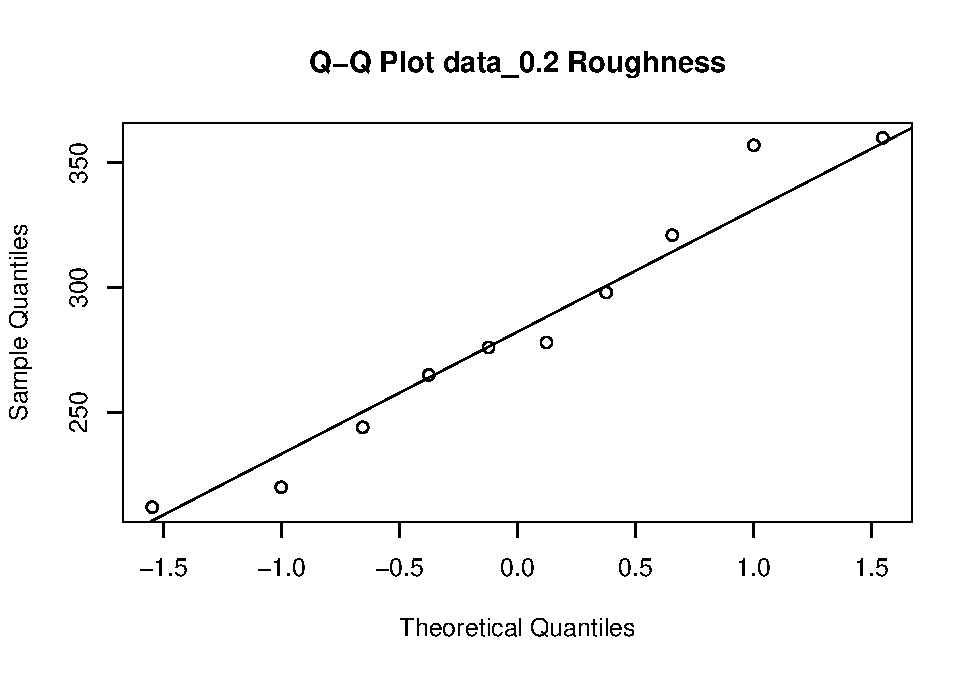
\includegraphics[keepaspectratio]{unnamed-chunk-28-1.pdf}}
    \caption{Đồ thị Q-Q Plot kiểm tra phân phối chuẩn tại chiều cao lớp in 0.2 mm}
    \label{fig:qq_layer_2}
\end{figure}
\newpage

\begin{Shaded}
\begin{Highlighting}[]
\FunctionTok{shapiro.test}\NormalTok{(data\_0}\FloatTok{.2}\SpecialCharTok{$}\NormalTok{roughness)}
\end{Highlighting}
\end{Shaded}

\begin{verbatim}
## 
##  Shapiro-Wilk normality test
## 
## data:  data_0.2$roughness
## W = 0.9451, p-value = 0.611
\end{verbatim}

Theo kết quả của code R, nhóm data có layer\_height là 0.1 và 0.15 không
tuân theo phân phối chuẩn, còn các nhóm còn lại tuân theo phân phối
chuẩn do có giá trị \texttt{p-value} lớn hơn mức ý nghĩa 5\%.

Điều kiện thứ ba: Phương sai ở các tổng thể phải bằng nhau.

Ta có:

\begin{itemize}
\item
  \(H_0\): Phương sai độ nhám ở các nhóm bằng nhau.
\item
  \(H_1\): Có ít nhất 2 nhóm có phương sai độ nhám khác nhau.
\end{itemize}

\emph{Ta dùng hàm leveneTest để tính toán các giá trị về phương sai.}

\begin{Shaded}
\begin{Highlighting}[]
\FunctionTok{library}\NormalTok{(car)}
\FunctionTok{leveneTest}\NormalTok{(roughness }\SpecialCharTok{\textasciitilde{}}\NormalTok{ layer\_height, data)}
\end{Highlighting}
\end{Shaded}

\begin{verbatim}
## Levene's Test for Homogeneity of Variance (center = median)
##       Df F value Pr(>F)
## group  4  1.4956 0.2195
##       45
\end{verbatim}

Ta thấy giá trị của \texttt{Pr(\textgreater{}F)\ =\ 0.2195} lớn hơn mức
ý nghĩa 5\%

\(\Rightarrow\) Chấp nhận \(H_0\), phương sai độ nhám ở các nhóm bằng nhau.

\textbf{Kết luận:} Ta thấy dữ liệu thỏa điều kiện thứ nhất, điều kiện
thứ ba nhưng ở điều kiện thứ hai còn một số nhóm data không thỏa mãn

\(\Rightarrow\) ANOVA trong dữ liệu này có thể mang tính chất tham khảo và có thể hoàn
toàn không chính xác.

\textbf{3.3. Phân tích sâu sau ANOVA (so sánh bội)}

\begin{Shaded}
\begin{Highlighting}[]
\FunctionTok{TukeyHSD}\NormalTok{(anova\_model)}
\end{Highlighting}
\end{Shaded}

\begin{verbatim}
##   Tukey multiple comparisons of means
##     95% family-wise confidence level
## 
## Fit: aov(formula = roughness ~ layer_height, data = data)
## 
## $layer_height
##            diff        lwr       upr     p adj
## 0.06-0.02  78.3   4.053227 152.54677 0.0341507
## 0.1-0.02  150.5  76.253227 224.74677 0.0000069
## 0.15-0.02 162.2  87.953227 236.44677 0.0000015
## 0.2-0.02  238.4 164.153227 312.64677 0.0000000
## 0.1-0.06   72.2  -2.046773 146.44677 0.0602239
## 0.15-0.06  83.9   9.653227 158.14677 0.0196501
## 0.2-0.06  160.1  85.853227 234.34677 0.0000020
## 0.15-0.1   11.7 -62.546773  85.94677 0.9914005
## 0.2-0.1    87.9  13.653227 162.14677 0.0130196
## 0.2-0.15   76.2   1.953227 150.44677 0.0416948
\end{verbatim}

\begin{Shaded}
\begin{Highlighting}[]
\FunctionTok{plot}\NormalTok{(}\FunctionTok{TukeyHSD}\NormalTok{(anova\_model))}
\end{Highlighting}
\end{Shaded}

\begin{figure}[htbp]
    \centering
    \pandocbounded{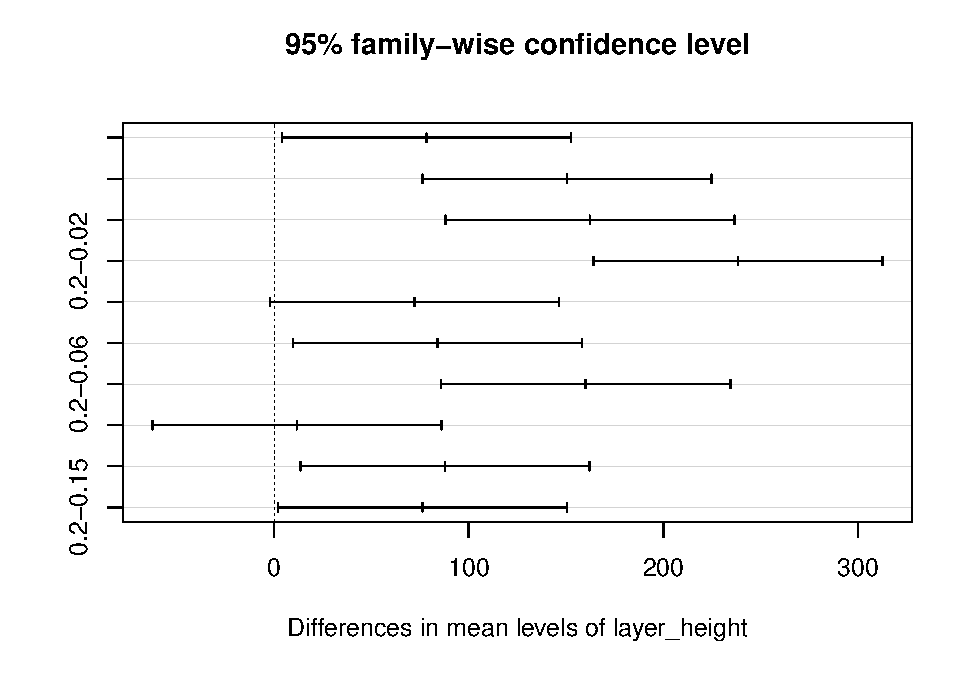
\includegraphics[keepaspectratio]{unnamed-chunk-30-1.pdf}}
    \caption{Đồ thị kiểm định hậu kiểm Tukey (Tukey HSD) cho các mức chiều cao lớp in}
    \label{fig:tukey_layer}
\end{figure}
\newpage

Ta có:

\begin{itemize}
\item
  \(H_0: \mu_i = \mu_j (i \neq j)\)
\item
  \(H_1: \mu_i \neq \mu_j (i \neq j)\)
\end{itemize}

Ta xét giá trị của \texttt{p-adj} nếu giá trị bé hơn mức ý nghĩa 5\% thì
sẽ bác bỏ \(H_0\) và chấp nhận \(H_1\)

Dựa vào giá trị sau khi tính toán hàm \texttt{TukeyHSD()} ta có: cặp giá
trị giữa \texttt{0.1\ –\ 0.06} và \texttt{0.15\ –\ 0.1} là lớn hơn mức ý
nghĩa 5\%

\(\Rightarrow\) Ta có: \(\mu_0.1 =\mu_0.6 %; %\mu_0.15 = \mu_0.1
\)

Bên cạnh đó, dựa trên các kết quả tính được, ta có thể sắp xếp theo thứ
tự giảm dần của các trung bình tổng thể như sau:
\(\mu_0.2>\mu_0.15=\mu_0.1>\mu_0.06>\mu_0.02\)

\textbf{Kết luận:} Muốn độ nhám thấp nhất thì \texttt{layer\_height}
cũng phải thấp nhất là \texttt{0.02}, muốn độ nhám giảm đi thì chiều cao
lớp in \texttt{layer\_height} cũng phải giảm đi.

\subsection*{4. Bài toán hồi quy tuyến tính đơn}

\textbf{Mô hình:} Hồi quy tuyến tính đa biến.

\textbf{Bài toán:} Phân tích mức độ ảnh hưởng của các thông số điều
chỉnh trong máy in 3D đến độ nhám (biến roughness) của bản in như thế
nào? Và dự báo thông số độ nhám của bản in dựa trên các thông số điều
chỉnh trong máy in 3D cho ngẫu nhiên.

\subsubsection*{4.1. Tính toán các giá trị, xây dựng và đánh giá mô hình}

\emph{Đây là code đi tính hồi quy tuyến tính của các biến theo độ nhám.}

\begin{Shaded}
\begin{Highlighting}[]
\NormalTok{model\_1 }\OtherTok{\textless{}{-}} \FunctionTok{lm}\NormalTok{(roughness }\SpecialCharTok{\textasciitilde{}}\NormalTok{ layer\_height }\SpecialCharTok{+}\NormalTok{ wall\_thickness }\SpecialCharTok{+}\NormalTok{ infill\_density }\SpecialCharTok{+}\NormalTok{ infill\_pattern }\SpecialCharTok{+}
\NormalTok{              nozzle\_temperature }\SpecialCharTok{+}\NormalTok{ bed\_temperature }\SpecialCharTok{+}\NormalTok{ print\_speed }\SpecialCharTok{+}\NormalTok{ material }\SpecialCharTok{+}\NormalTok{ fan\_speed,} 
\NormalTok{              new\_data)}
\FunctionTok{summary}\NormalTok{(model\_1)}
\end{Highlighting}
\end{Shaded}

\begin{verbatim}
## 
## Call:
## lm(formula = roughness ~ layer_height + wall_thickness + infill_density + 
##     infill_pattern + nozzle_temperature + bed_temperature + print_speed + 
##     material + fan_speed, data = new_data)
## 
## Residuals:
##     Min      1Q  Median      3Q     Max 
## -72.746 -24.332  -1.641  20.304  96.552 
## 
## Coefficients: (1 not defined because of singularities)
##                           Estimate Std. Error t value Pr(>|t|)    
## (Intercept)             -2.371e+03  3.716e+02  -6.379 1.25e-07 ***
## layer_height             1.269e+03  8.765e+01  14.483  < 2e-16 ***
## wall_thickness           2.334e+00  2.189e+00   1.066  0.29259    
## infill_density          -4.231e-02  2.341e-01  -0.181  0.85742    
## infill_patternhoneycomb -1.255e-01  1.128e+01  -0.011  0.99117    
## nozzle_temperature       1.506e+01  2.529e+00   5.953 5.05e-07 ***
## bed_temperature         -1.613e+01  3.251e+00  -4.962 1.27e-05 ***
## print_speed              6.496e-01  2.060e-01   3.153  0.00302 ** 
## materialpla              2.985e+02  5.836e+01   5.114 7.78e-06 ***
## fan_speed                       NA         NA      NA       NA    
## ---
## Signif. codes:  0 '***' 0.001 '**' 0.01 '*' 0.05 '.' 0.1 ' ' 1
## 
## Residual standard error: 38.24 on 41 degrees of freedom
## Multiple R-squared:  0.8752, Adjusted R-squared:  0.8509 
## F-statistic: 35.95 on 8 and 41 DF,  p-value: 3.834e-16
\end{verbatim}

\emph{Phát hiện biến \texttt{fan\_speed} có hệ số NA → có đa cộng tuyến}

Kiểm tra đa cộng tuyến

\emph{Ta sử dụng thư viện corrplot để mô hình hóa ma trận tương quan
giữa các biến với nhau.}

\begin{Shaded}
\begin{Highlighting}[]
\NormalTok{data\_filter}\OtherTok{\textless{}{-}}\NormalTok{new\_data[, }\FunctionTok{c}\NormalTok{(}\StringTok{"layer\_height"}\NormalTok{, }\StringTok{"wall\_thickness"}\NormalTok{, }\StringTok{"infill\_density"}\NormalTok{, }
\StringTok{"nozzle\_temperature"}\NormalTok{, }\StringTok{"bed\_temperature"}\NormalTok{, }\StringTok{"print\_speed"}\NormalTok{, }\StringTok{"fan\_speed"}\NormalTok{, }\StringTok{"roughness"}\NormalTok{)]}

\NormalTok{cor\_data}\OtherTok{\textless{}{-}}\FunctionTok{cor}\NormalTok{(data\_filter)}
\FunctionTok{corrplot}\NormalTok{(cor\_data)}
\end{Highlighting}
\end{Shaded}

\begin{figure}[htbp]
    \centering
    \pandocbounded{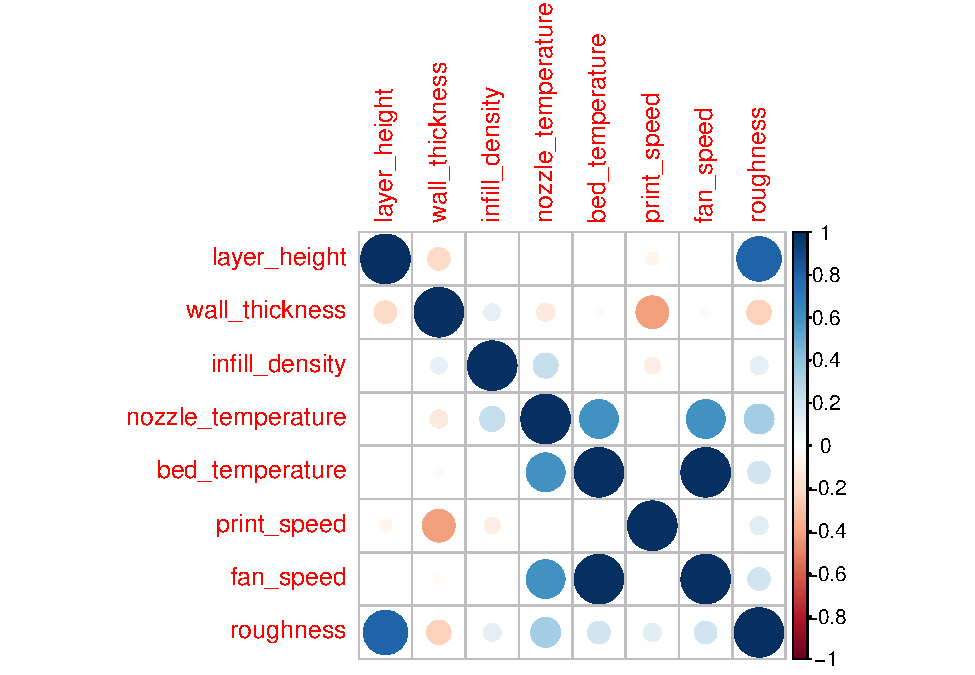
\includegraphics[keepaspectratio]{unnamed-chunk-32-1.pdf}}
    \caption{Biểu đồ ma trận tương quan giữa các biến điều chỉnh định lượng}
    \label{fig:corrplot}
\end{figure}
\newpage

Ta dễ dàng nhìn thấy giữa biến bed\_temperature và fan\_speed có 2 vòng
tròn xanh đậm, chứng tỏ có mối quan hệ tuyến tính mạnh với nhau.

\textbf{Kết luận:} Loại bỏ biến \texttt{fan\_speed}.

Chạy lại mô hình hồi quy sau khi loại bỏ biến \texttt{fan\_speed}

\begin{Shaded}
\begin{Highlighting}[]
\NormalTok{model\_1 }\OtherTok{\textless{}{-}} \FunctionTok{lm}\NormalTok{(roughness }\SpecialCharTok{\textasciitilde{}}\NormalTok{ layer\_height }\SpecialCharTok{+}\NormalTok{ wall\_thickness }\SpecialCharTok{+}\NormalTok{ infill\_density }\SpecialCharTok{+}\NormalTok{ infill\_pattern }\SpecialCharTok{+}
\NormalTok{              nozzle\_temperature }\SpecialCharTok{+}\NormalTok{ bed\_temperature }\SpecialCharTok{+}\NormalTok{ print\_speed }\SpecialCharTok{+}\NormalTok{ material , new\_data)}
\FunctionTok{summary}\NormalTok{(model\_1)}
\end{Highlighting}
\end{Shaded}

\begin{verbatim}
## 
## Call:
## lm(formula = roughness ~ layer_height + wall_thickness + infill_density + 
##     infill_pattern + nozzle_temperature + bed_temperature + print_speed + 
##     material, data = new_data)
## 
## Residuals:
##     Min      1Q  Median      3Q     Max 
## -72.746 -24.332  -1.641  20.304  96.552 
## 
## Coefficients:
##                           Estimate Std. Error t value Pr(>|t|)    
## (Intercept)             -2.371e+03  3.716e+02  -6.379 1.25e-07 ***
## layer_height             1.269e+03  8.765e+01  14.483  < 2e-16 ***
## wall_thickness           2.334e+00  2.189e+00   1.066  0.29259    
## infill_density          -4.231e-02  2.341e-01  -0.181  0.85742    
## infill_patternhoneycomb -1.255e-01  1.128e+01  -0.011  0.99117    
## nozzle_temperature       1.506e+01  2.529e+00   5.953 5.05e-07 ***
## bed_temperature         -1.613e+01  3.251e+00  -4.962 1.27e-05 ***
## print_speed              6.496e-01  2.060e-01   3.153  0.00302 ** 
## materialpla              2.985e+02  5.836e+01   5.114 7.78e-06 ***
## ---
## Signif. codes:  0 '***' 0.001 '**' 0.01 '*' 0.05 '.' 0.1 ' ' 1
## 
## Residual standard error: 38.24 on 41 degrees of freedom
## Multiple R-squared:  0.8752, Adjusted R-squared:  0.8509 
## F-statistic: 35.95 on 8 and 41 DF,  p-value: 3.834e-16
\end{verbatim}

Lúc này kết quả đã không còn hiện tượng đa cộng tuyến.

\(\Rightarrow\) Phương trình hồi quy tuyến tính có dạng:

\emph{Y = B\_1.layer\_height+B\_2.wall\_thickness+\ldots{}}

\textbf{Đánh giá:} Phương trình tổng quát thì không tìm được chỉ có thể
thông qua 1 bộ dữ liệu mẫu và ở đây là dữ liệu với 50 lần quan sát nên
chỉ có thể có phương trình ước lượng mà thôi.

\(\Rightarrow\) Phương trình hồi quy tuyến tính ước lượng có dạng:

\emph{Y =B\_1.layer\_height+B\_2.wall\_thickness+\ldots{}}

Muốn kiểm định xem các thông số của máy in 3D có ảnh hưởng như thế nào
đến với độ nhám của lớp in hay không, ta đi kiểm định hệ số của từng
thông số, nếu hệ số = 0 thì thông số không có ảnh hưởng đến với độ nhám
của lớp in và ngược lại.

Ta có:

\begin{itemize}
\item
  \(H_0: B_i=0\)
\item
  \(H_1: B_i≠0\)
\end{itemize}

\textbf{Ta sẽ đi so sánh:} \texttt{p-value} =
Pr(\textgreater\textbar t\textbar) nếu nhỏ hơn mức ý nghĩa 5\% thì sẽ
bác bỏ \(H_0\) và chấp nhận \(H_1\). Khi đó thông số có giá trị
\texttt{p-value} nhỏ hơn mức ý nghĩa 5\% sẽ có ảnh hưởng đến với độ nhám
của lớp in và ngược lại.

Dựa vào bảng giá trị ở trên, ta thấy có 3 thông số là: wall\_thickness,
infill\_density và infill\_pattern là có \texttt{p-value} lớn hơn mức ý
nghĩa 5\% , chứng tỏ chấp nhận \(H_0\): \(B_i=0\)

\(\Rightarrow\) 3 thông số đó không có ảnh hưởng đến độ nhám của lớp in.

\(\Rightarrow\) 3 thông số sẽ được loại bỏ khỏi mô hình.

\textbf{Ta xét đến yếu tố:}

\begin{itemize}
\item
  \(R^2\) : Thể hiện phần trăm biến động của độ nhám lớp in được giải
  thích bởi biến độc lập có trong mô hình.
\item
  \(R^2\) có phạm vi từ 0 đến 1. Càng tiến về 1 thì chứng tỏ mô hình
  giải thích rất tốt đối với sự biến động của độ nhám lớp in do những
  biến độc lập (thông số máy in 3D) gây ra.
\end{itemize}

\textbf{Đánh giá: } Đối với mô hình hồi quy tuyến tính đa bội thì khi
đánh giá mô hình ta sẽ dựa vào thông số \(R^2\) hiệu chỉnh (Adjusted
R-squared) để đánh giá mô hình mà không sử dụng thông số \(R^2\)

\textbf{Giải thích: } Do đối với thông số \(R2\) thì cứ mỗi lần cung cấp
1 biến độc lập vào mô hình thì thông số \%R2\% sẽ tăng mà không quan tâm
biến độc lập đó có vi phạm điều kiện gì hay không.

\(\Rightarrow\) Dẫn đến nếu cung cấp các biến độc lập nhưng không ảnh hưởng đến mô
hình vào thì lúc này thông số \(R2\) sẽ không còn đáng tin cậy nữa.

Vì vậy đối với mô hình hồi quy tuyến tính đa bội, khi đánh giá mô hình
sẽ dựa vào thông số \(R^2\) hiệu chỉnh để đánh giá vì thông số \(R2\)
hiệu chỉnh sẽ cân bằng lại so với việc khi đưa nhiều biến độc lập không
ảnh hưởng tới mô hình.

\emph{Ta bắt đầu xây dựng mô hình sau khi đã loại bỏ 3 biến không ảnh
hưởng đến mô hình.}

\begin{Shaded}
\begin{Highlighting}[]
\NormalTok{model\_2 }\OtherTok{\textless{}{-}} \FunctionTok{lm}\NormalTok{(roughness }\SpecialCharTok{\textasciitilde{}}\NormalTok{ layer\_height }\SpecialCharTok{+}\NormalTok{ nozzle\_temperature }\SpecialCharTok{+}\NormalTok{ bed\_temperature }
\SpecialCharTok{+}\NormalTok{ print\_speed }\SpecialCharTok{+}\NormalTok{ material, }\AttributeTok{data =}\NormalTok{ new\_data)}
\FunctionTok{summary}\NormalTok{(model\_2)}
\end{Highlighting}
\end{Shaded}

\begin{verbatim}
## 
## Call:
## lm(formula = roughness ~ layer_height + nozzle_temperature + 
##     bed_temperature + print_speed + material, data = new_data)
## 
## Residuals:
##     Min      1Q  Median      3Q     Max 
## -74.084 -26.500  -1.662  22.585  92.356 
## 
## Coefficients:
##                      Estimate Std. Error t value Pr(>|t|)    
## (Intercept)        -2310.7356   353.2009  -6.542 5.38e-08 ***
## layer_height        1246.5353    83.1780  14.986  < 2e-16 ***
## nozzle_temperature    14.7774     2.3979   6.163 1.95e-07 ***
## bed_temperature      -15.8078     3.0895  -5.117 6.55e-06 ***
## print_speed            0.5538     0.1804   3.070  0.00366 ** 
## materialpla          294.1610    56.1586   5.238 4.38e-06 ***
## ---
## Signif. codes:  0 '***' 0.001 '**' 0.01 '*' 0.05 '.' 0.1 ' ' 1
## 
## Residual standard error: 37.44 on 44 degrees of freedom
## Multiple R-squared:  0.8717, Adjusted R-squared:  0.8571 
## F-statistic: 59.78 on 5 and 44 DF,  p-value: < 2.2e-16
\end{verbatim}

Lúc này ta thấy giá trị của \(R2\) hiệu chỉnh đã tăng hơn so với ban đầu
và lớn hơn 0.8 chứng tỏ mô hình đang khá tốt.

\emph{Ta sẽ dự đoán mô hình dựa trên những giá trị ngẫu nhiên của các
biến độc lập (các thông số của máy in 3D) }

\begin{Shaded}
\begin{Highlighting}[]
\NormalTok{data\_test }\OtherTok{\textless{}{-}} \FunctionTok{data.frame}\NormalTok{(}\AttributeTok{layer\_height =} \FloatTok{0.03}\NormalTok{, }\AttributeTok{nozzle\_temperature =} \DecValTok{250}\NormalTok{, }
\AttributeTok{bed\_temperature =} \DecValTok{80}\NormalTok{, }\AttributeTok{print\_speed =} \DecValTok{80}\NormalTok{, }\AttributeTok{material =} \StringTok{"abs"}\NormalTok{)}
\NormalTok{data\_test}\SpecialCharTok{$}\NormalTok{predicted\_value }\OtherTok{\textless{}{-}} \FunctionTok{predict}\NormalTok{(model\_2, }\AttributeTok{newdata =}\NormalTok{ data\_test, }
\AttributeTok{interval =} \StringTok{"confidence"}\NormalTok{, }\AttributeTok{level =} \FloatTok{0.95}\NormalTok{)}
\FunctionTok{print}\NormalTok{(data\_test)}
\end{Highlighting}
\end{Shaded}

\begin{verbatim}
##   layer_height nozzle_temperature bed_temperature print_speed material
## 1         0.03                250              80          80      abs
##   predicted_value.fit predicted_value.lwr predicted_value.upr
## 1            200.7033            167.2929            234.1136
\end{verbatim}

\subsubsection*{4.2. Đánh giá các điều kiện của mô hình hồi quy }

\emph{Ta sẽ dùng hàm plot() để đánh giá các điều kiện của mô hình hiện
tại.}

\begin{Shaded}
\begin{Highlighting}[]
\FunctionTok{par}\NormalTok{(}\AttributeTok{mfrow =} \FunctionTok{c}\NormalTok{(}\DecValTok{2}\NormalTok{, }\DecValTok{2}\NormalTok{))}
\FunctionTok{plot}\NormalTok{(model\_2)}
\end{Highlighting}
\end{Shaded}

\begin{figure}[htbp]
    \centering
    \pandocbounded{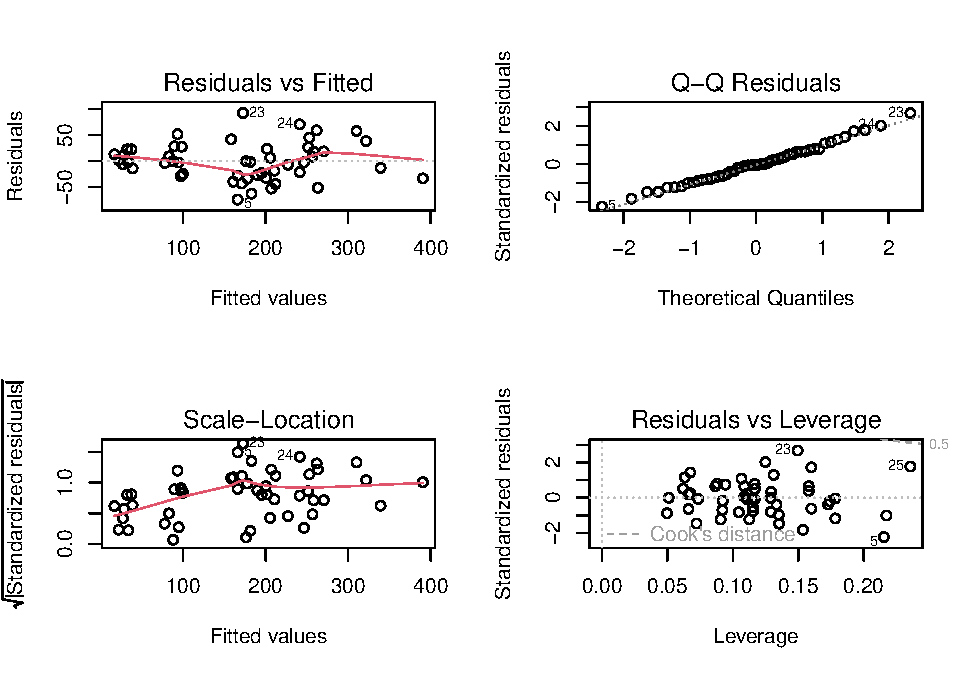
\includegraphics[keepaspectratio]{unnamed-chunk-36-1.pdf}}
    \caption{Các đồ thị phân tích thặng dư đánh giá điều kiện của mô hình hồi quy}
    \label{fig:model_diagnostics}
\end{figure}
\newpage

\textbf{Điều kiện thứ nhất: Sai số phải tuân theo phân phối chuẩn.}

Ta sẽ dựa vào đồ thị Q-Q Residuals để đánh giá.

Ta thấy các điểm trên hình tập trung gần với đường thẳng phân phối chuẩn

\(\Rightarrow\) Sai số tuân theo phân phối chuẩn.

\(\Rightarrow\) Thỏa mãn điều kiện thứ nhất.

\textbf{Điều kiện thứ hai: Sai số có kì vọng bằng 0.}

Ta sẽ dựa vào đồ thị Residuals vs Fitted để đánh giá.

Nếu đường màu đỏ nằm gần đường bằng 0 thì có thể nói sai số có kì vọng
bằng 0.

Ở đây ta thấy đường màu đỏ không nằm sát đường bằng 0

\(\Rightarrow\) Mô hình có sai số có kì vọng khác 0.

\(\Rightarrow\) Vi phạm điều kiện thứ hai.

\textbf{Điều kiện thứ ba: Phương sai của các sai số là hằng số (sai số
đồng nhất)}

Nếu những điểm này nó phân bố ngẫu nhiên dọc theo đường màu đỏ

\(\Rightarrow\) Ta nói phương sai của các sai số là hằng số

Nhưng khi nhìn vào đồ thị của hình thì ta thấy nó chỉ phân bố tập trung
nhiều ở đoạn đầu đường màu đỏ và khu vực giữa đường đỏ

\(\Rightarrow\) Vi phạm điều kiện thứ ba.

\textbf{Điều kiện thứ tư: Không có hiện tượng đa cộng tuyến xảy ra.}

Ở đây model\_2 đã được loại bỏ các biến gây nên hiện tượng đa cộng tuyến

\(\Rightarrow\) Thỏa mãn điều kiện thứ tư.

\textbf{Điều kiện thứ năm: Các sai số độc lập với nhau.}

Ta sử dụng biểu đồ Residuals vs Index.

\begin{Shaded}
\begin{Highlighting}[]
\FunctionTok{plot}\NormalTok{(}\FunctionTok{residuals}\NormalTok{(model\_2), }\AttributeTok{type =} \StringTok{"b"}\NormalTok{, }\AttributeTok{main =} \StringTok{"Residuals vs Index"}\NormalTok{,}
    \AttributeTok{xlab =} \StringTok{"Index"}\NormalTok{, }\AttributeTok{ylab =} \StringTok{"Residuals"}\NormalTok{)}
\FunctionTok{abline}\NormalTok{(}\AttributeTok{h =} \DecValTok{0}\NormalTok{, }\AttributeTok{col =} \StringTok{"red"}\NormalTok{)}
\end{Highlighting}
\end{Shaded}

\begin{figure}[htbp]
    \centering
    \pandocbounded{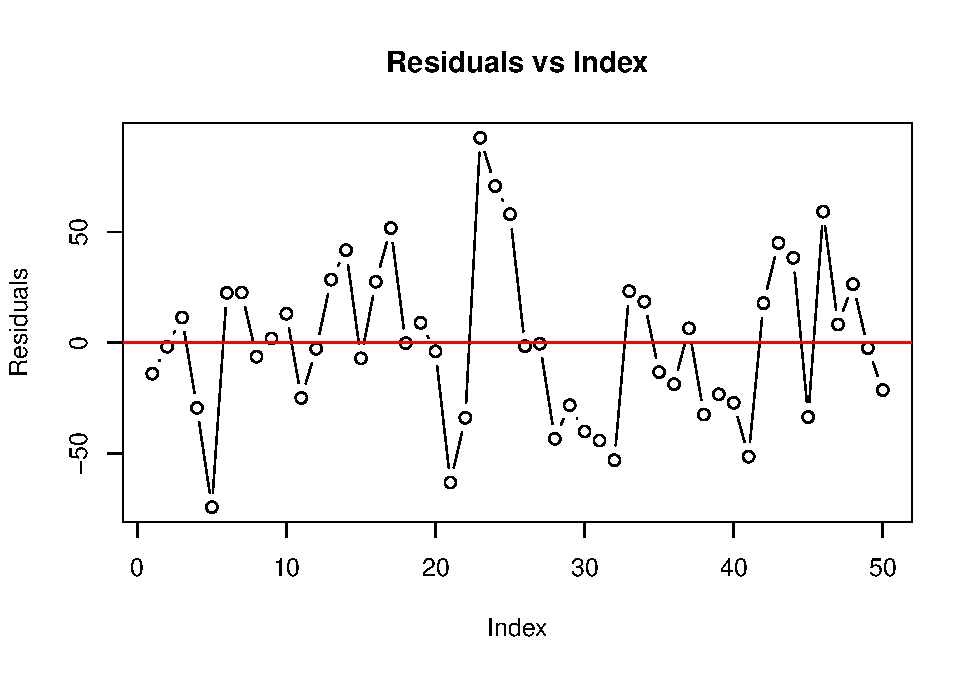
\includegraphics[keepaspectratio]{unnamed-chunk-37-1.pdf}}
    \caption{Biểu đồ kiểm tra tính độc lập của các sai số (Residuals vs Index)}
    \label{fig:residuals_index}
\end{figure}
\newpage

Dựa trên mô hình kết quả, ta thấy các điểm phân bố theo ngẫu nhiên mà
không có một quy tắc rõ ràng.

\(\Rightarrow\) Các sai số độc lập với nhau.

\(\Rightarrow\) Thỏa mãn điều kiện thứ năm.
\newpage